\subsubsection{La Contrôleur}
\label{subsubsec:controleur}

Afin de garantir le bon fonctionnement de notre application, nous avons implémenté un contrôleur qui permet de gérer les interactions entre les différentes parties de notre application. Le contrôleur est composé de plusieurs classes qui permettent de gérer les différents menus, les paramètres audio, les règles du jeu, la création de partie, la partie en elle-même, etc. C'est ce qui lie notre MVC et permet de faire fonctionner notre application.

\paragraph{Les mouvements}

% TODO: Parler des controleurs de mouvements

\paragraph{Les menus}

\paragraph{L'écran d'accueil}

Nous avons un écran d'accueil, géré par la classe StartMenu.java, qui possède des boutons pour:

\begin{itemize}
    \item Aller au menu de création de partie (Bouton Start)
    \item Aller au menu des paramètres audio (Bouton Engrenage)
    \item Afficher les règles du jeu (Bouton Start)
          %   \item Afficher les crédits
          % \item Quitter le jeu
\end{itemize}

Les différents éléments graphiques tels que le GIF et les images des boutons sont gérés par la classe JPanelWithImages.java.

\begin{figure}[h!]
    \centering
    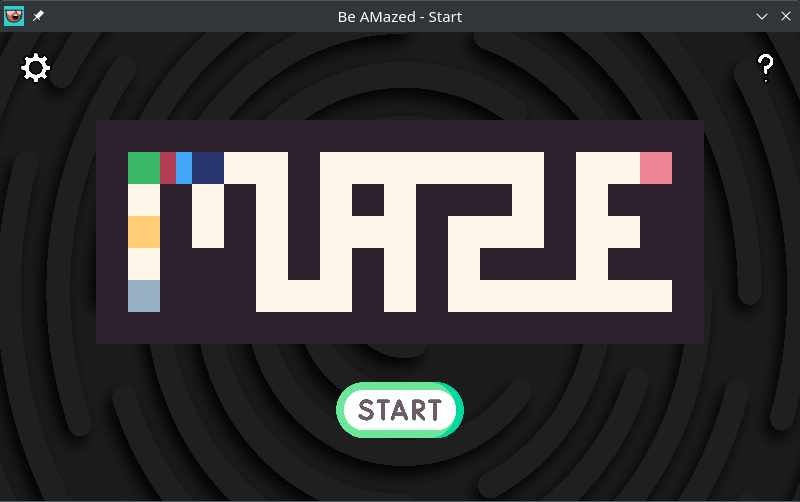
\includegraphics[scale=0.4]{ressources/Implementation/Labyrinthe/Controleur/StartMenu.png}%
    \caption{L'écran d'accueil}
    \label{fig:StartMenu}
\end{figure}

\paragraph{Les paramètres audio}

La vue des paramètres audio sera abordée dans la section \ref{subsec:son}.

\paragraph{Les règles de jeu}

Les règles du jeu sont affichées en anglais dans une fenêtre qui se superpose à celle du menu principal.

\begin{figure}[h!]
    \centering
    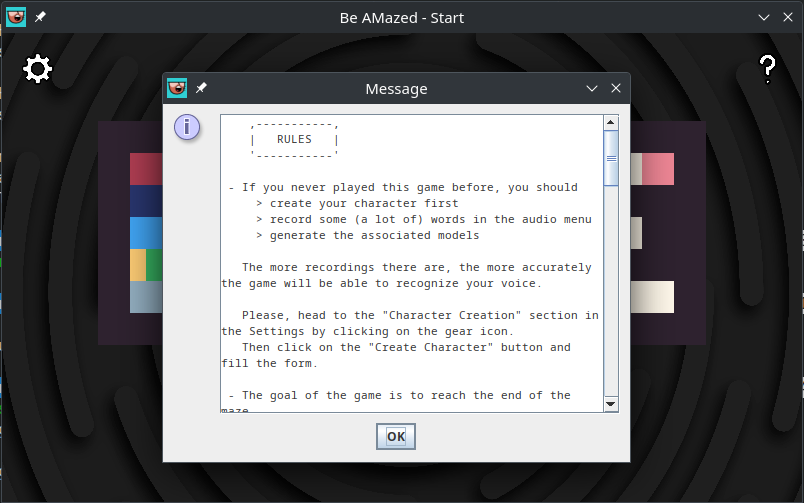
\includegraphics[scale=0.4]{ressources/Implementation/Labyrinthe/Controleur/Rules.png}%
    \caption{Les règles du jeu}
    \label{fig:Rules}
\end{figure}

\paragraph{La création de partie}

La création de la partie se décompose en plusieurs étapes et dispose de plusieurs éléments graphiques afin de permettre à l'utilisateur de choisir les paramètres de la partie qu'il souhaite jouer (nombre de joueurs, difficulté, etc.) le plus facilement possible. Cela est rendu possible par la classe SettingsMenu.java qui gère l'ensemble des menus de paramétrage de la partie.

\subparagraph*{Le choix du mode de jeu}

Le menu déroulant permet de choisir entre les différents modes de jeu disponibles. Il est géré par la classe SelectionPanel.java.

\begin{figure}
    \centering
    \subfloat{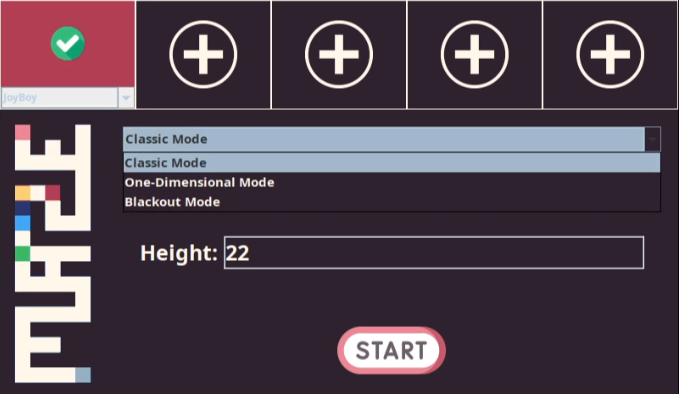
\includegraphics[scale=0.5]{ressources/Implementation/Labyrinthe/Controleur/SettingsMenu_ModeList.png}}%
    \caption{Menu déroulant des modes de jeu}
    \label{fig:ModeSelection}
\end{figure}

Pour les afficher les menus des différents modes de jeu, nous avons des classes qui permettent de gérer les différents panels concernés. Ces classes sont des implémentations de l'interface PanelHandler.java et sont créées grâce à la classe PanelHandlerFactory.java.

\subparagraph*{Le mode Classique}

Avec la classe ClassicPanelHandler.java, nous avons à disposition deux entrées textes permettent de choisir la taille du labyrinthe.

\begin{figure}
    \centering
    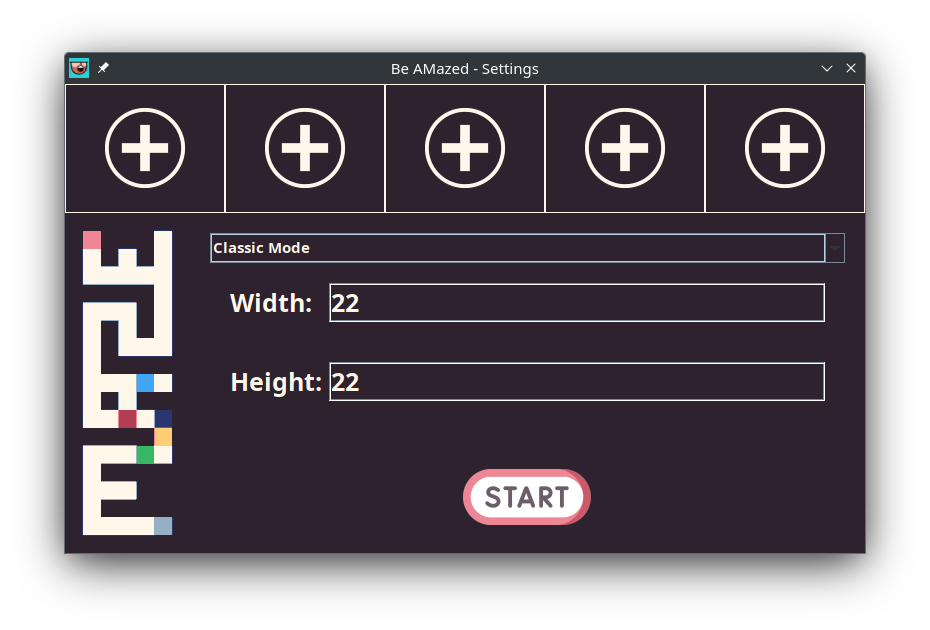
\includegraphics[scale=0.5]{ressources/Implementation/Labyrinthe/Controleur/SettingsMenu_ClassicMode.png}
    \caption{Paramètres du mode classique}
    \label{fig:ClassicMode}
\end{figure}